To assess the usefulness and effectiveness of our approach, we developed a prototype tool that implements \zop\ and performed an empirical evaluation on several software benchmarks. (For simplicity, in this section we use the name \zop\ to refer to both the approach and its implementation, unless otherwise stated.) In our evaluation, we quantified (1) the accuracy of the profiling information computed by \zop and (2) how the training inputs used affect \zop's accuracy. In the rest of this section, we discuss our implementation of \zop, our evaluation setup, and the results of our evaluation.

% The first research question assesses how the \zop\ profiling results
% compare to profiling results from existing profiling techniques. The
% second research question explores the impact that the number of
% training examples of a path has on the profiling accuracy for that
% path.

\subsection{ZOP Implementation} 
\label{sec:implementation-1}

For our evaluation, we used a NIOS II processor on an Altera Cyclone II FPGA. This processor has many of the features of modern complex computer systems (\eg a 32 bit RISC MIPS-like architecture, a large external DRAM, separate instruction and data caches, dynamic branch prediction) while also providing features that were extremely useful for developing our understanding of how program execution affects the system's EM emanations (\eg programmable digital I/O pins, access to programmable logic, and cycle-accurate program tracing). For the evaluation, we did not use any FPGA-specific features.

We leveraged LLVM~\cite{LLVM} to detect the acyclic paths in the code, identify instrumentation points, and insert instrumentation. We then used LLVM's C backend to generate instrumented C source code. GCC then compiled this source code to a NIOS binary. Both the original and instrumented source code are standard C code and could be compiled and run on any modern architecture.

The software parts of \zop are built using freely available software (\ie compiler, code analysis framework, and FPGA tools). To observe EM emanations, we used a magnetic field probe (a small inductor in series with a tuning capacitor) that was placed directly over the processor's decoupling capacitors. The EM probe was assembled by hand by one of the authors from components that can be bought for less than \$10. Finally, we used a spectrum analyzer (which can be a fairly expensive piece of equipment) to demodulate and record EM emanations so as to have more control and flexibility in our investigation, but numerous software defined radio receivers, which are available for less than \$1,000 have sufficient capability and precision to reproduce our measurements.

\subsection{Evaluation Setup}
\label{sec:evaluation-setup}
\begin{table}[htb]
  \begin{center}
    \caption{Statistics for the SIR benchmark profiled by ZOP.}
    \begin{tabular}{|c|c|c|c|c|}
      \hline
      Benchmark & LOC & Markers
      & Training Set Size
      & Profiling Set Size \\
%      & \multicolumn{1}{m{0.4in}|}{\centering Path \\ Profiling \\ Accuracy}  \\
      \hline
      \hline
      print\_tokens & 571 & 48 & 240 & 400 \\
      \hline
      schedule      & 415 & 36 & 284 & 400 \\
      \hline
      replace       & 563 & 54 & 299 & 400 \\
      \hline
      Total        & 1549 &138 & 823 & 1200 \\
      \hline
    \end{tabular}
    \label{table:benchmarks}
  \end{center}
\end{table}

We selected three programs in the SIR repository~\cite{Software-artifact} to profile: replace, print\_tokens, and schedule. Table~\ref{table:benchmarks} shows, for each benchmark, its name, its size, the number of markers added during training, and the number of inputs we used during the training and profiling phases.

%5)Reviewer1/Reviewer2:How would ZOP scale to more/larger programs?
%We were limited by slow/general-purpose measurement equipment and
%manual effort for porting benchmarks and inputs. 
The decision to use only a few relatively small benchmarks was largely due to limitations of the system we used and of our measurement setup.  The runtime we used in our evaluation, for instance, does not have an operating system. To automate measurements, we thus had to modify the standalone programs we profiled so that their \texttt{main()} function was called repeatedly from a wrapper executable. Because standalone programs tend to depend on data memory being initialized to zero when \texttt{main()} is called and typically do not clean up memory before exiting, this introduced issues that required manual effort for each program. Furthermore, we had to use LLVM's C backend to generate instrumented C code that was recompiled on the target system (in a real application \zop\ would directly instrument binaries), which also created problems and required extensive manual checking. In addition, our general purpose measurement setup resulted in long measurement times, which favored the use of shorter executions of smaller programs. In general, avoiding larger programs allowed us to perform fairly extensive manual checks of our results, which helped us gain confidence in their correctness and, most importantly, let us get a deeper understanding of the issues involved in our approach and how to address them. 

%6)Reviewer2:Is the use of high-coverage inputs for training required?
%Training does not need coverage of all paths, as long as it observed
%the branches on these paths a few times. Production-quality software
%often has coverage-adequate test suites. Most importantly, even
%executions of individual procedures (e.g., through
%much-easier-to-create unit tests) should provide enough information
%for training.  
%9)Reviewer1:We separated training and testing sets to
%make sure our *testing* set had good path coverage (which we believe
%made the evaluation more challenging for ZOP than selecting multiple
%random cross-validation sets).
We selected the inputs for profiling and training as follows. For profiling, we selected inputs that achieved high path coverage, so as to demonstrate that \zop\ can accurately profile a large number of different paths. As for the training set, ideally we would want an input set that exercises all the possible behaviors (in terms of EM emissions) of marker-to-marker subpaths; \zop\ would then be able to identify complete paths by concatenating these short subpaths. As a more realistic proxy for this set, we selected training inputs that achieved branch coverage and then added a random set of extra inputs (see next paragraph). It is worth noting that production-quality software often already provides test suites with high branch coverage.  Most importantly, for the purpose of training, much-easier-to-create unit tests for individual procedures could also be used.

Specifically, we performed our input selection by starting with the existing set of inputs in the SIR repository~\cite{Software-artifact}.  For each benchmark, we randomly split the inputs for that benchmark into two equally-sized disjoint sets: \textit{training superset} and \textit{profiling supersets}. This guarantees that the inputs used for training are completely independent of those used for profiling. From the training superset, we randomly selected a minimal subset of inputs that achieved the same branch coverage as the complete set. We then added 150 extra inputs randomly selected from the superset to increase the chances of having different paths covered by different numbers of inputs, so as to be able to study how the characteristics of the training inputs affect \zop's accuracy and determine how the training inputs affect profiling accuracy. We selected 150 as the number of extra training inputs based on earlier experiments, as that number is not excessively large and yet can provide a higher variety in coverage. We call the resulting set the \textit{training set}. To determine the set of inputs for profiling (\ie the \textit{profiling set}), we randomly selected a subset of the profiling superset that achieved the same acyclic-path coverage as the complete set and then added random inputs to get to 400 inputs, which was the largest number of inputs we could measure in the amount of time we had available.

\begin{figure}[htb]
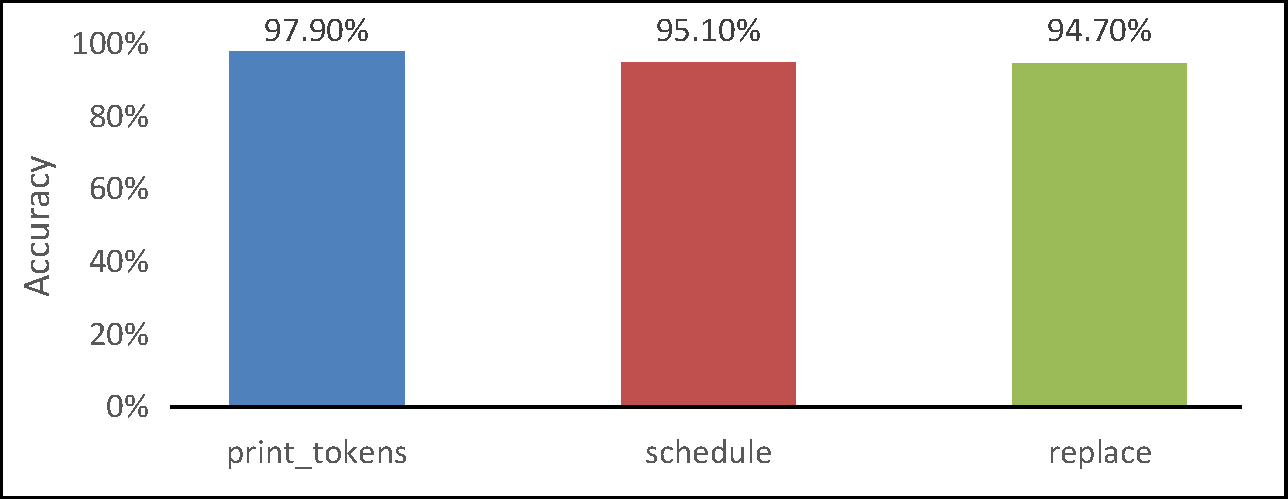
\includegraphics[width=5in]{../issta_profile/profiling/figures/overall-correctness}
\caption{Average accuracy per benchmark.}
\label{fig:overall_correctness}
\end{figure}

\subsection{Results}

To quantify \zop's accuracy, we first determined the path taken for each profiled input (\ie the ground truth) by measuring the correct profiling information for each benchmark and each input in the profiling set. Because \zop\ estimates profiling at the acyclic-path level, we used the approach by Ball and Larus~\cite{Ball:1996:EPP:243846.243857} to compute this information. Next, we performed \zop's Training~1, Training~2, and Profiling phases. For each benchmark and each profiled input, \zop\ predicted the number of times each acyclic path was executed, and we compared this value with the previously computed ground truth. We then calculated the average accuracy for each benchmark using the following formula:

\[\textrm{accuracy} = \frac{\sum_{i=1}^{n}g_{i} a_{i}}{\sum_{i=1}^{n}g_{i}}\]

where 
% SPACE
\begin{align*}
  n = & \textrm{~number of acyclic paths per benchmark.} \\
  g_i = & \textrm{~actual number executions of acyclic path~} i
          \textrm{(ground truth)}. \\
  z_i = & \textrm{~\zop~(predicted) number of executions of acyclic path~} i. \\
  a_{i} = & \textrm{~min} \Big (\frac{g_i}{z_i}, \frac{z_i}{g_i} \Big)
            = \textrm{~accuracy for acyclic path~} i. \\
\end{align*}

Therefore, when \zop\ underestimates the number of executions of a path, the accuracy is computed as $a_i = \frac{z_i}{g_i}$, whereas when \zop\ overestimates the number of executions of a path, the accuracy is computed as $a_i = \frac{g_i}{z_i}$. $a_i = 0$ when $z_i=0$. To give equal weight to each path execution, each $a_i$ is weighted by $g_i$.

Figure~\ref{fig:overall_correctness} shows the path profiling accuracy results. As the table shows, \zop's estimates are fairly accurate.  On average, \zop\ correctly predicts 94.7\% of the paths for replace, 97.9\% for print\_tokens, and 95.1\% for schedule. In other words, the profiling information computed by \zop\ \textit{without any instrumentation} is always over 94\% accurate.

Determine how the coverage of training inputs affects ZOP's accuracy, we computed how the accuracy of \zop's path count estimates is affected by the number of times each path is exercised by the training set. We show these results in Figure~\ref{fig:all_benchmarks}.  Each data point in this figure represents the accuracy of \zop's estimate for a single static acyclic path in the indicated benchmark (\ie a single $a_i$ value). For each benchmark, the figure also shows a fit for a saturating power curve\footnote{The curve is $y=a-bx^c$ where $x$ is the number of dynamic instances, $y$ is accuracy, and $a$, $b$, and $c$ are constants chosen (for each benchmark separately) to produce the best fit.} for each benchmark and the curve's goodness of fit (\ie $R^2$). We chose this type of curve because, among all simple curves we tried, including linear, quadratic, exponential, etc. it produces (by far) the best goodness-of-fit.  A logarithmic scale is used for the x-axis to more directly show the effect of increasing the number of training path instances by an order of magnitude.

\begin{comment}
\begin{figure}[htb]
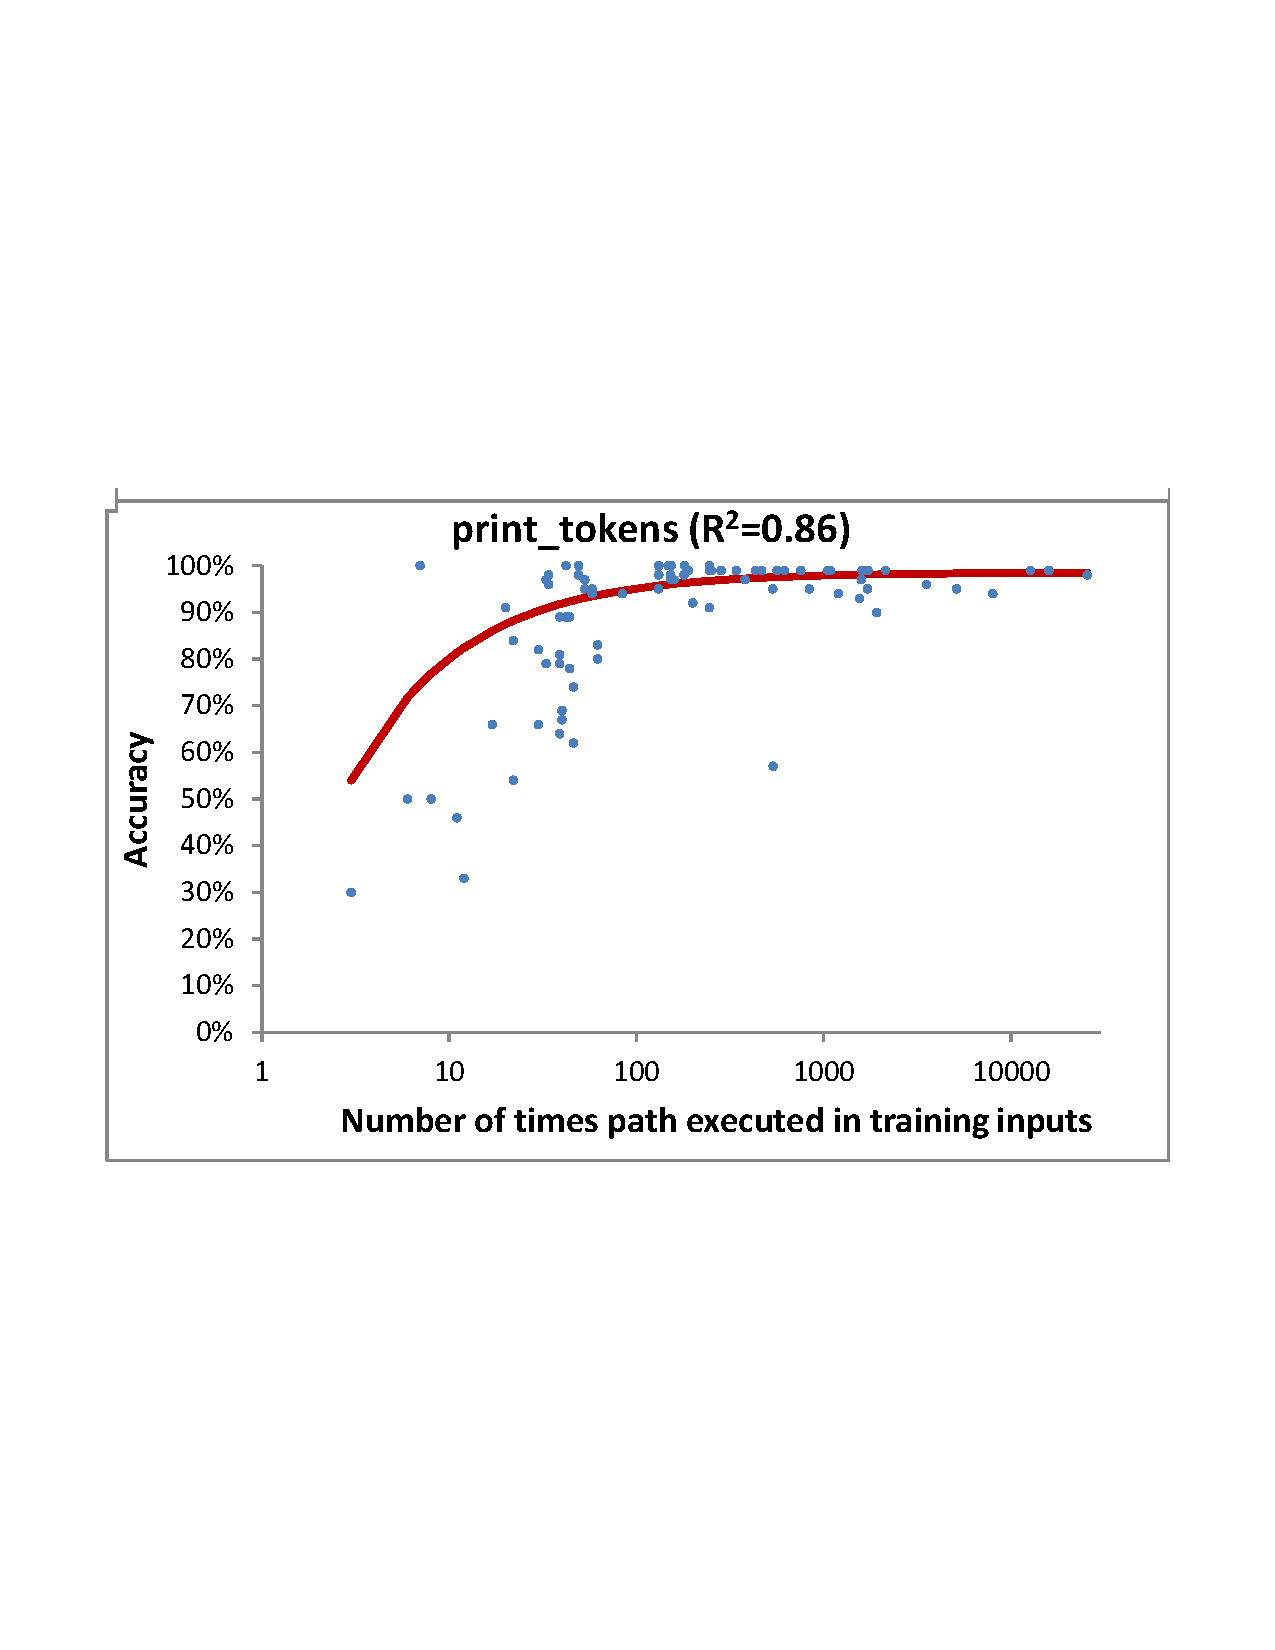
\includegraphics[width=5in]{../issta_profile/profiling/figures/print_tokens}
% SPACE \caption{Effect of the number of training examples on accuracy for print\_tokens.}
\caption{Number of training examples vs accuracy for print\_tokens.}
\label{fig:print_tokens}
\end{figure}

\begin{figure}[hbt]
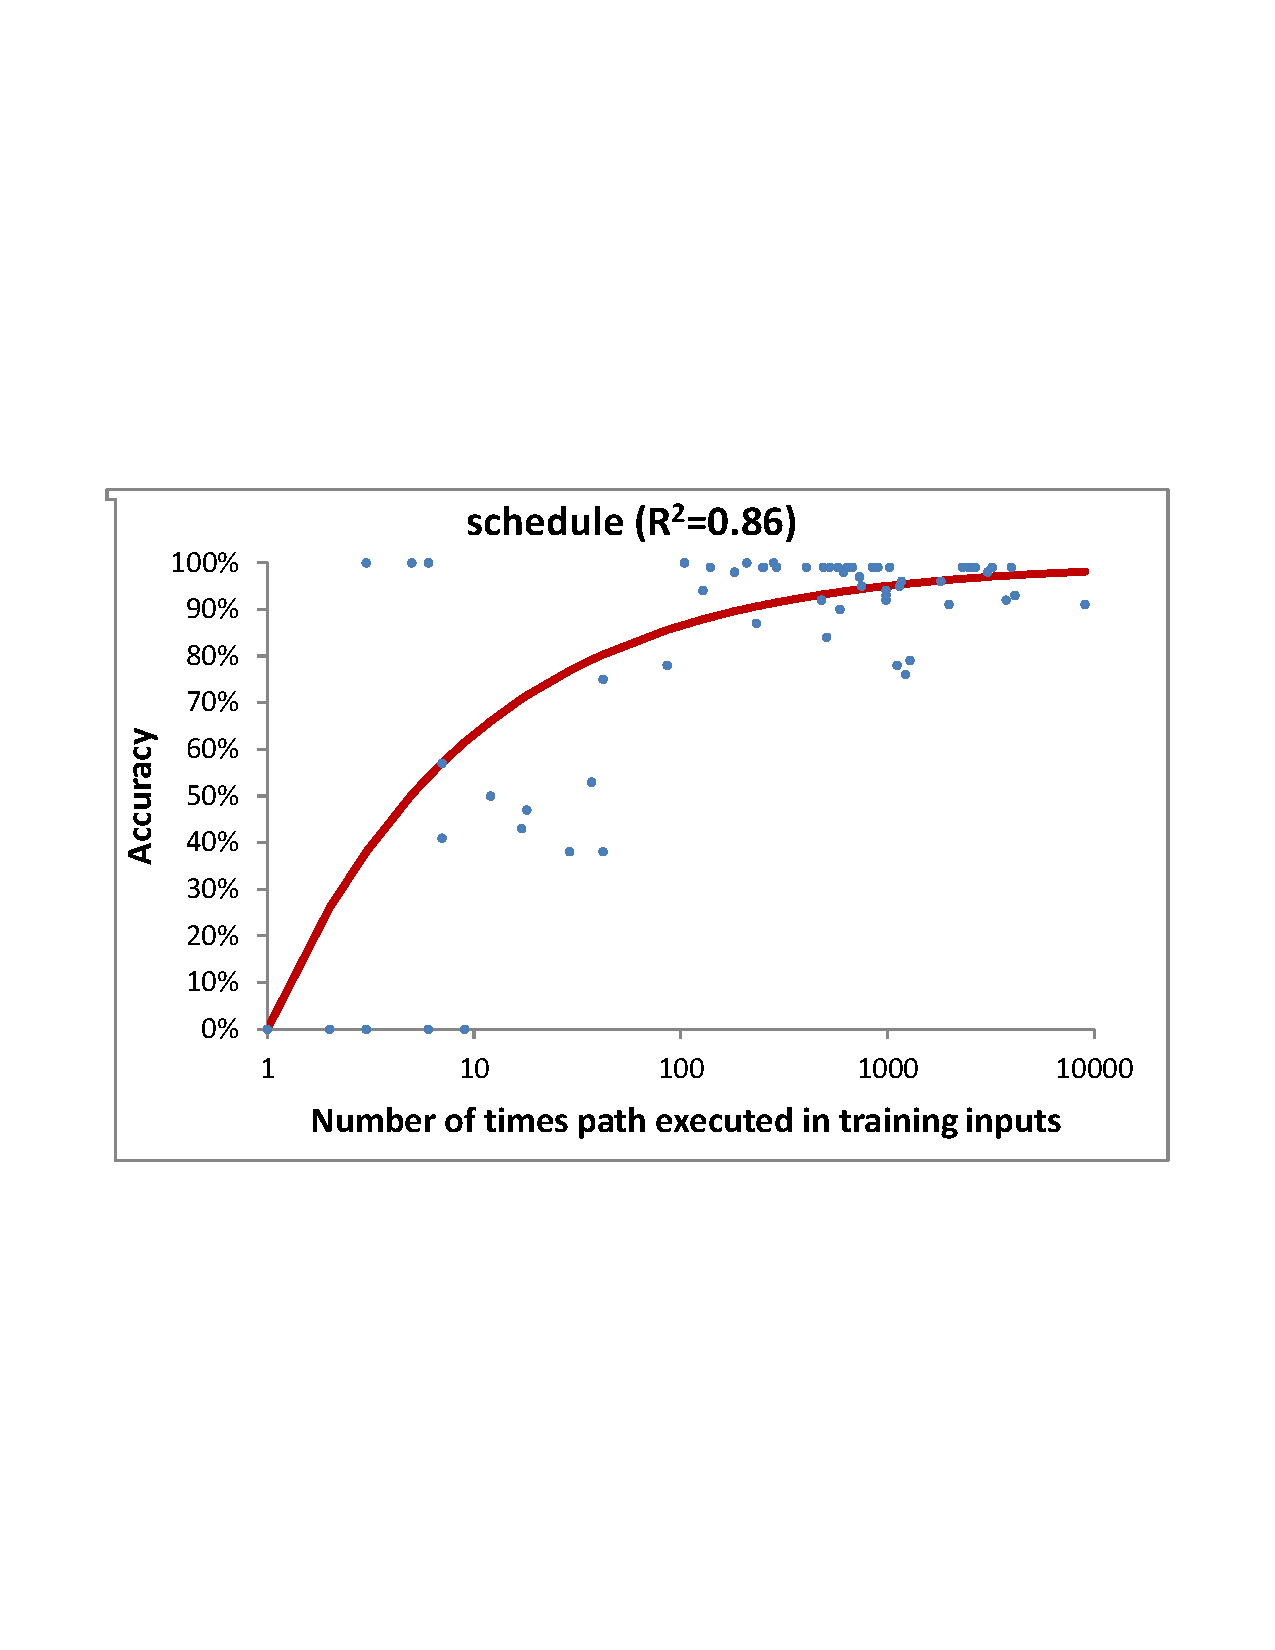
\includegraphics[width=5in]{../issta_profile/profiling/figures/schedule}
%\caption{Effect of the number of training examples on accuracy for schedule.}
\caption{Number of training examples vs accuracy for schedule.}
\label{fig:schedule}

\end{figure}

\begin{figure}[hbt]
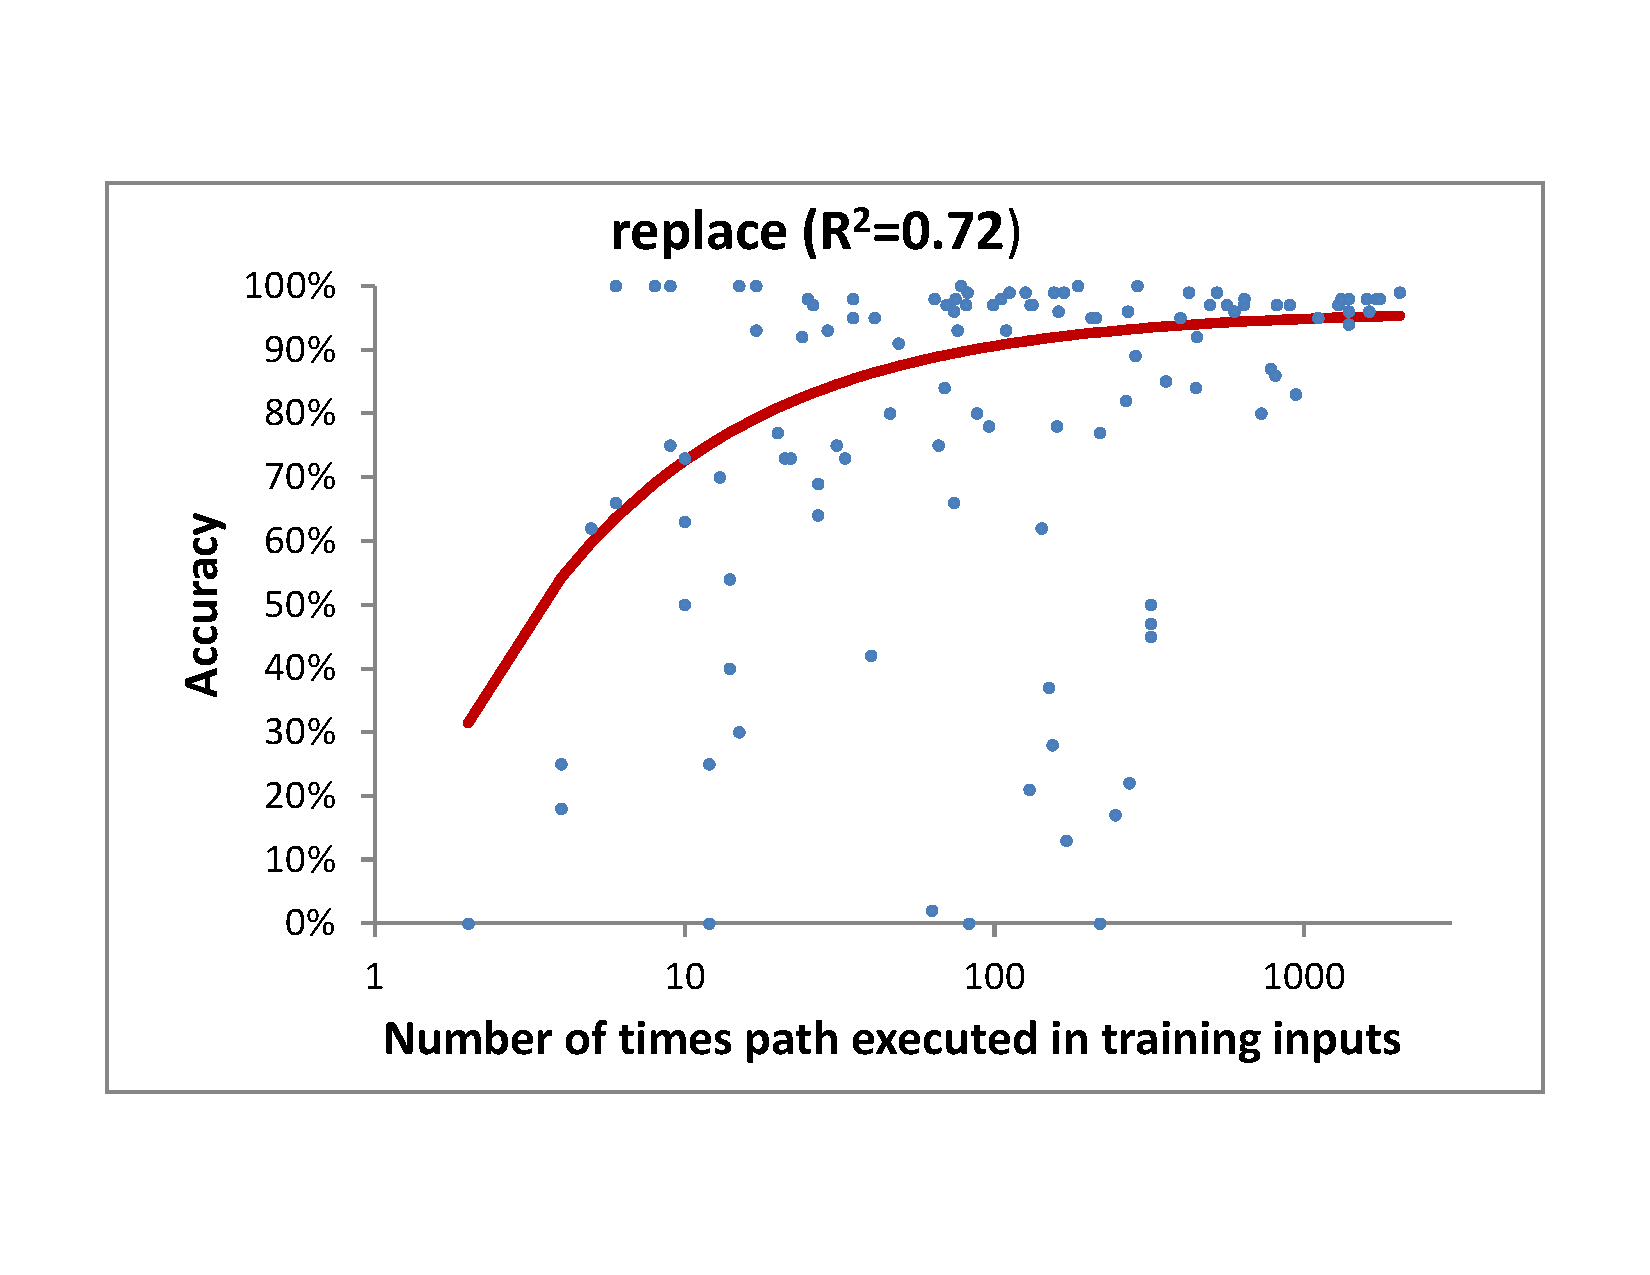
\includegraphics[width=5in]{../issta_profile/profiling/figures/replace}
% SPACE \caption{Effect of the number of training examples on accuracy for replace.}
\caption{Number of training examples vs accuracy for replace.}
\label{fig:replace}
\end{figure}
\end{comment}


\begin{figure*}[bt]

\includegraphics[width=\textwidth]{../issta_profile/profiling/figures/all_benchmarks}
% SPACE \caption{Effect of the number of training examples on accuracy for replace.}
\caption{Number of training examples vs accuracy for print\_tokens, schedule, and replace.}
\label{fig:all_benchmarks}
\end{figure*}

For the print\_tokens and schedule benchmarks in Figure~\ref{fig:all_benchmarks}, the accuracy is poor when the acyclic path is executed less than 100 times, but greatly improves beyond this point.  In fact, the vast majority of paths with more than 100 occurrences during training have nearly perfect accuracy.  This is promising, as it implies that paths can be identified accurately by a relatively small number of inputs that cover them. Moreover, it also implies that accuracy can be improved by adding more training inputs.  Finally, as we said in Section~\ref{sec:evaluation-setup}, even executions of individual procedures by means of unit tests (which are easier to create) should be sufficient for training.

The replace benchmark manifests a slightly different behavior. While the accuracy does increase with the number of times the paths are covered during training, there are several paths with more than 100 training examples that have accuracy below 80\%, and even a few below 50\%. In general the accuracy for replace does not improve as quickly as for the other two benchmarks as a function of the number of executions of a path during training.

We investigated this difference in behavior and found several possible explanations. First, whereas we expect most paths to have only so many variations in terms of the EM emanations that they can generate (see Section~\ref{zop-background}), some paths may vary more widely based on the context in which they are executed. Alternatively, some paths may simply have more possible contexts under which they can be executed (\eg if the structure of the program or some parts thereof contains especially high levels of nesting).
% I removed the discussion about interprocedural because it did not
% convince me and, moreover, contradicted the idea of using unit
% tests, which I believe can be promising...

Second, the path prediction algorithm traverses a program's marker graph as shown in the example in Figure~\ref{fig:backtracking}. This traversal results in the evaluation (and possibly selection) of many impossible paths. The technique that we use to navigate the graph is context sensitive but does not distinguish between different call sites that invoke the same callee from within a procedure. Therefore, the algorithm could reach a callee from a given call site within a procedure and return to a different call site within the same procedure. This is particularly problematic in programs in which this situation occurs frequently and may lead to imprecision and poor predictions.
%(the above issue does clearly impact performance). If further investigation confirms that this issue is indeed present, we will suitably increase the precision of our algorithm.

Finally, for 3 of the 400 inputs in replace's profiling set, the path prediction algorithm got ``lost'' while exploring the marker graph. As we mentioned while describing our approach, if the waveforms collected during training do not closely match the waveform collected during profiling for more than a short time, the predicted and actual control flows can diverge beyond recovery. Once this happens, the remainder of the prediction for that input is completely incorrect. This condition only happened for the replace benchmark and only for three inputs. This is likely an indication that there is something different about replace and that more training inputs were needed for certain parts of this benchmark. Also in this case, we will perform further investigation to better characterize the peculiarities of replace and use our findings to improve \zop.
